\documentclass[a4paper,AutoFakeBold,12pt]{ctexbook}
\usepackage[top=3cm,bottom=2.5cm,left=3cm,right=2cm]{geometry}
\usepackage{graphicx,subfig}  
\linespread{1}
%%此文档用于引用所需package

\usepackage[%paperwidth=18.4cm, paperheight= 26cm,  % 版面控制宏包,定义规定的版面尺寸
            body={14.5true cm,21true cm}       %论文版芯145mm×210mm(包括页眉及页码则为145mm×230mm)
                               %页码在版芯下边线之下隔行居中放置;
            %headheight=1.0true cm
            ]{geometry}
\usepackage{layouts}				% 打印当前页面格式的宏包
\usepackage[sf]{titlesec}			% 控制标题的宏包
\usepackage{titletoc}				% 控制目录的宏包
\usepackage[perpage,symbol]{footmisc}   % 脚注控制
\usepackage{fancyhdr}				% fancyhdr宏包 页眉和页脚的相关定义
\usepackage{fancyref}        
   
\usepackage{CJK}			% 中文支持宏包
\usepackage{type1cm}		% tex1cm宏包,控制字体的大小
\usepackage{times}			% 使用Times字体的宏包
\usepackage{indentfirst}	% 首行缩进宏包
\usepackage{color}			% 支持彩色 % 引用的宏包
\graphicspath{{figures/}} 

%-----------------------标题格式---------------------------------
\usepackage{caption}
\captionsetup{font={footnotesize}}%宋体小5,居中
\usepackage{titlesec}

% \arabic 罗马数字  \alph 小写字母 \Alph 大写字母  \roman 小写罗马数字 \Roman 大写罗马数字 \chinese{section} 一、二 
\CTEXsetup[format+={\songti\bfseries\zihao{-3}},number={\arabic{chapter}},name={第,章},afterskip={\baselineskip},beforeskip={-.5\baselineskip}]{chapter}%一级标题 小3宋体加粗、居中   afterskip以及beforeskip还需要确认。,afterskip={34pt},beforeskip={-6pt}
\CTEXsetup[format+={\heiti\bfseries\zihao{-4}\raggedright},beforeskip={.5\baselineskip},afterskip={.5\baselineskip}]{section}%二级标题 小4黑体,居左,afterskip={13pt},beforeskip={13pt}
\CTEXsetup[format={\songti\zihao{-4}\raggedright},beforeskip={.5\baselineskip},afterskip={.5\baselineskip}]{subsection}%三级标题 小4宋体居左,afterskip={13pt},beforeskip={13pt}

\usepackage{fontspec} 
\setCJKmainfont{SimSun} %正文字体宋体  SimHei 黑体
\setmainfont{Times New Roman} %英文字符 新罗马字体

\usepackage{fancyhdr}


\newtheorem{theorem}{\hspace{2em}定理}[section]
\newtheorem{definition}{\hspace{2em}定义}[section]
\newtheorem{lemma}{\hspace{2em}引理}[section]
\newtheorem{corollary}{\hspace{2em}推论}[section]
\newtheorem{proposition}{\hspace{2em}性质}[section]
\newtheorem{example}{\hspace{2em}例}[section]
\newtheorem{remark}{\hspace{2em}注}[section]


%------------------------ Abstract & Keywords -------------------------
\newcommand\cntitle{中文题目}
\newcommand\entitle{English Title}
\newcommand\cnkeywordsname{关键词}
\newcommand\cnkeywords[1]{ {\noindent\heiti\cnkeywordsname: }#1}
\newcommand\enkeywordsname{Key Words}
\newcommand\enkeywords[1]{ {\noindent\bfseries\enkeywordsname: }#1}
\newenvironment{cnabstract}{%
    \newpage
    \chapter{{\cntitle}}				%会使与摘要之间空格由afterskip控制。
    \centerline{\songti\zihao{-3} 摘~~~~要}%自由控制
         \vskip 30pt
        \par
    \setlength{\parindent}{24bp}
    }{}
\newenvironment{enabstract}{%
    \newpage
    \centerline{\bfseries\zihao{-3} \entitle}
    \vskip 10bp
    \centerline{\bfseries\zihao{-3} ABSTRACT}
         \vskip 30bp
        \par
    \setlength{\parindent}{24bp}
    }{}


\begin{document}
%------------------------------前言之前部分的页面格式---------------------------
\pagestyle{fancy}%此部分设计摘要、英文摘要、目录清单、前言页面风格。
\fancyhead[CO]{\small{安徽工程大学毕业设计(论文)}}%单页页眉
\fancyhead[CE]{\small{张玉动:基于Android的模拟炒股APP}}%双页页眉
\fancyhead[R,L]{}
\fancyfoot[C]{\thepage}%页脚
\pagenumbering{Roman}%页码以罗马格式书写
%%======中文摘要===========================%
\begin{cnabstract}
本篇文档主要介绍{\bf 北航毕业设计论文\LaTeX{}模板}使用和相关软件环境的安装配置,
以及本模板所遵循的开源协议等。

本篇文档主要介绍{\bf 北航毕业设计论文\LaTeX{}模板}使用和相关软件环境的安装配置,
以及本模板所遵循的开源协议等。
\end{cnabstract}
\newline
\cnkeywords{毕业论文; \LaTeX{}; 模板;  }

%%======英文摘要===========================%
\begin{enabstract}
本篇文档主要介绍{\bf 北航毕业设计论文\LaTeX{}模板}使用和相关软件环境的安装配置,
以及本模板所遵循的开源协议等。

本篇文档主要介绍{\bf 北航毕业设计论文\LaTeX{}模板}使用和相关软件环境的安装配置,
以及本模板所遵循的开源协议等。
\end{enabstract}
\newline
\enkeywords{毕业论文; \LaTeX{}; 模板;  }


\newpage
%------------------------------------前言之后的页面格式-------------------------
\pagestyle{fancy}%此部分设置正文以及附录部分页面风格。
\fancyhead[CO]{\small{安徽工程大学毕业设计(论文)}}
\fancyhead[CE]{\small{张玉动:基于Android的模拟炒股APP}}
\fancyhead[R,L]{}
\fancyfoot[C]{-\thepage-}
\pagenumbering{arabic}
\assignpagestyle{\chapter}{fancy}    %该命令将chapter自带的pagestyle设置为fancy
\chapter*{前言}
\chapter{第一章}
\chapter{第二章}
\section{你好了}
\section{我}
\subsection{三级标题}
二级标题
\subsection{三级标题}
三级标题\newline
\begin{tabular}{ll}
 \verb|\songti| & {\songti 宋体} \\
 \verb|\heiti| & {\heiti 黑体} \\
 \verb|\fangsong| & {\fangsong 仿宋} \\
 \verb|\kaishu| & {\kaishu 楷书}
\end{tabular}
\begin{tabular}{ll}
\verb|\zihao{0}| &\zihao{0}  初号字 English \\
\verb|\zihao{-0}|&\zihao{-0} 小初号 English \\
\verb|\zihao{1} |&\zihao{1}  一号字 English \\
\verb|\zihao{-1}|&\zihao{-1} 小一号 English \\
\verb|\zihao{2} |&\zihao{2}  二号字 English \\
\verb|\zihao{-2}|&\zihao{-2} 小二号 English \\
\verb|\zihao{3} |&\zihao{3}  三号字 English \\
\verb|\zihao{-3}|&\zihao{-3} 小三号 English \\
\verb|\zihao{4} |&\zihao{4}  四号字 English \\
\verb|\zihao{-4}|&\zihao{-4} 小四号 English \\
\verb|\zihao{5} |&\zihao{5}  五号字 English \\
\verb|\zihao{-5}|&\zihao{-5} 小五号 English \\
\verb|\zihao{6} |&\zihao{6}  六号字 English \\
\verb|\zihao{-6}|&\zihao{-6} 小六号 English \\
\verb|\zihao{7} |&\zihao{7}  七号字 English \\
\verb|\zihao{8} |&\zihao{8}  八号字 English \\
\end{tabular}
wftc \\
\begin{table}[ht]
\centering
\caption{一般三线表}
\label{tab:1}
    \begin{tabular}{c c c c c c c c c c c}
    \hline
    123 & 4  & 5  & 123 & 4 & 5123 & 4 & 5 & 123 & 4 & 5\\
    \hline
    67 & 890 & 13 & 123 & 4 & 5123 & 4 & 5 & 123 & 4 & 5\\
    67 & 890 & 13 & 123 & 4 & 5123 & 4 & 5 & 123 & 4 & 5\\
    67 & 890 & 13 & 123 & 4 & 5123 & 4 & 5 & 123 & 4 & 5\\
    \hline
    \end{tabular}
\end{table}
这是一个图表\\
\begin{theorem}
海明码是广泛采用的一种有效的检验码,它实际上是一种多重奇偶校验码,其实原理在有效信息位中加入几个检验位形成海明码。
\end{theorem}

\begin{figure}[tbp]
	\centering
	\subfloat[Arabic numerals]{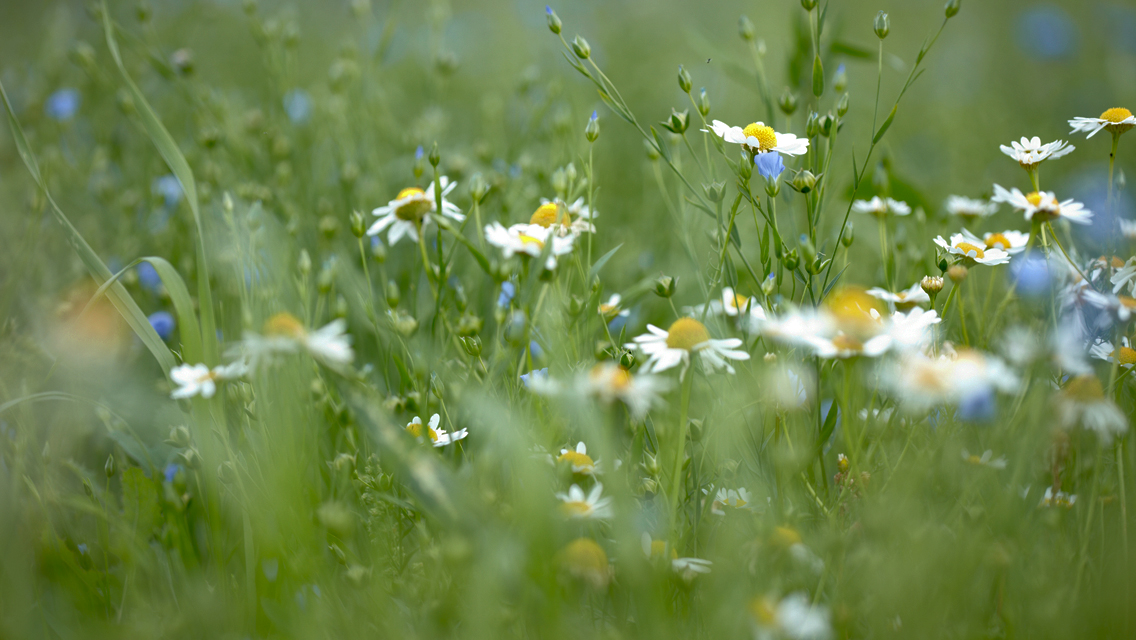
\includegraphics[width=3in]{Daisy.jpg}}\quad
	\subfloat[Arabic numerals]{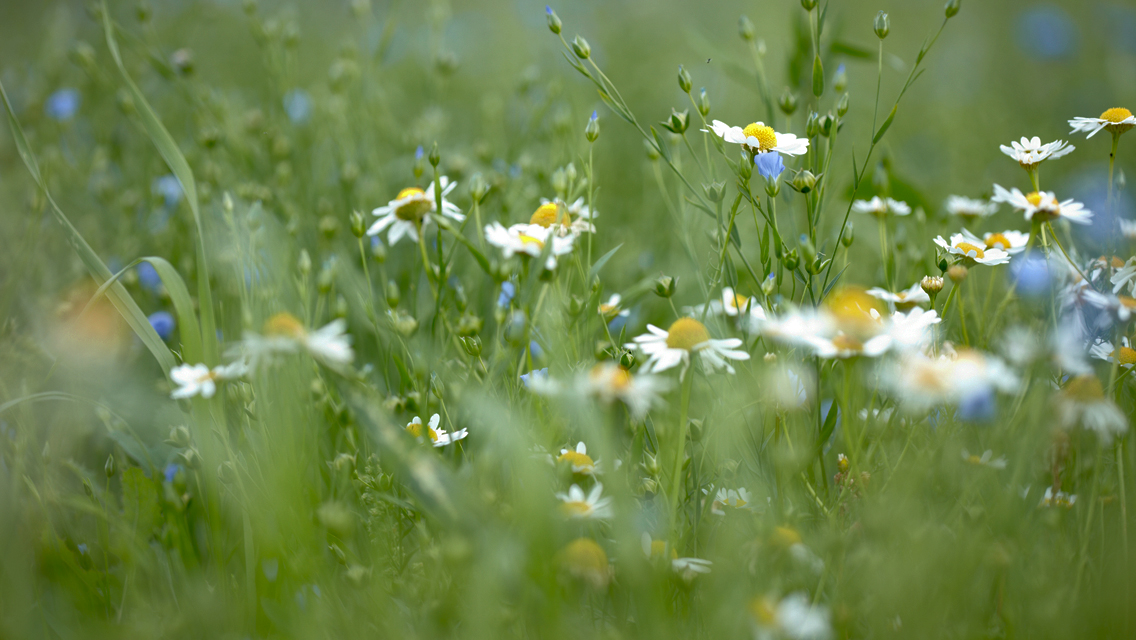
\includegraphics[width=3in]{Daisy.jpg}}\\	
	\caption{Capital Roman numerals.}
\end{figure}
\newpage
你好了
\newpage
这篇通用latex论文模板仅为兴趣而生,为学习而发热。编写过程中阅读了大量的package,但latex并非一个可以系统学习的软件。所以在学习的过程中我借鉴了大量的其它大学的论文模板,而加以合适的改造,进而对latex这个typeset系统有了进一步的了解。但是目前仍旧对底层代码不熟悉,由于当下的时间和精力问题,这个学习方向只能交给将来的我是否有时间和兴趣了。
\end{document}
